% TEX compiler = latexmk
% copyright arturo salinas-aguayo 2024
\documentclass[12pt]{article}

\usepackage{graphicx}
\usepackage{amsmath}
\usepackage{array}
\usepackage{amsfonts}
\usepackage{fancyhdr}
\usepackage{geometry}
\usepackage{circuitikz}
\usepackage{subfigure}
\usepackage{caption}
\usepackage{karnaugh-map}
\usepackage{bm}
\usepackage[table]{xcolor}
\usepackage{float}

\geometry{letterpaper, margin=1in}
\graphicspath{ {../images/} }

% Header and Footer
\pagestyle{fancy}
\fancyhf{}
\fancyhead[L]{CSE 2301 - Lab 08: The Voting Machine}
\fancyhead[R]{\thepage}
\setlength{\headheight}{15pt}

\author{Arturo Salinas-Aguayo}
\title{Lab 08: The Voting Machine}
% theorem set
\newtheorem{example}{Example}
% Example block environment
\newenvironment{examp}
{
	\vspace{.5cm}
	\hrule
\begin{example}\upshape}
	{\hrule
		\vspace{0.5cm}
\end{example}}

\begin{document}
\newcommand{\closure}[2][3]{%
	{}\mkern#1mu\overline{\mkern-#1mu#2}}
\newcommand\ncoverline[1]{\mkern1mu\overline{\mkern-1mu#1\mkern-1mu}\mkern1mu}
% Title Page
\begin{titlepage}
	\centering
	\vspace*{3cm}
	\huge\textbf{Lab 08: The Voting Machine}\\
	\vspace{5cm}
	\Large\textbf{Arturo Salinas-Aguayo}\\
	\normalsize
	CSE 2301: Principles and Practice of Digital Logic Design\\
	Dr. Mohammad Khan, Section 003L-1248\\
	Electrical and Computer Engineering Department
	\vfill
	
\includegraphics[scale=0.1]{uconnlogo}\\
	College of Engineering, University of Connecticut\\
	\scriptsize{Coded in \LaTeX}
	\vspace*{1cm}
\end{titlepage}
\section*{Theory}
\subsubsection*{What is a Multiplexor?}
A Multiplexor allows the designer to choose from several possible inputs based
on the value of a \textit{select} signal.
The output is selected by the select signal. For example, for a 4:1 MUX has four
data inputs and one output.
\begin{figure}[H]
	\center{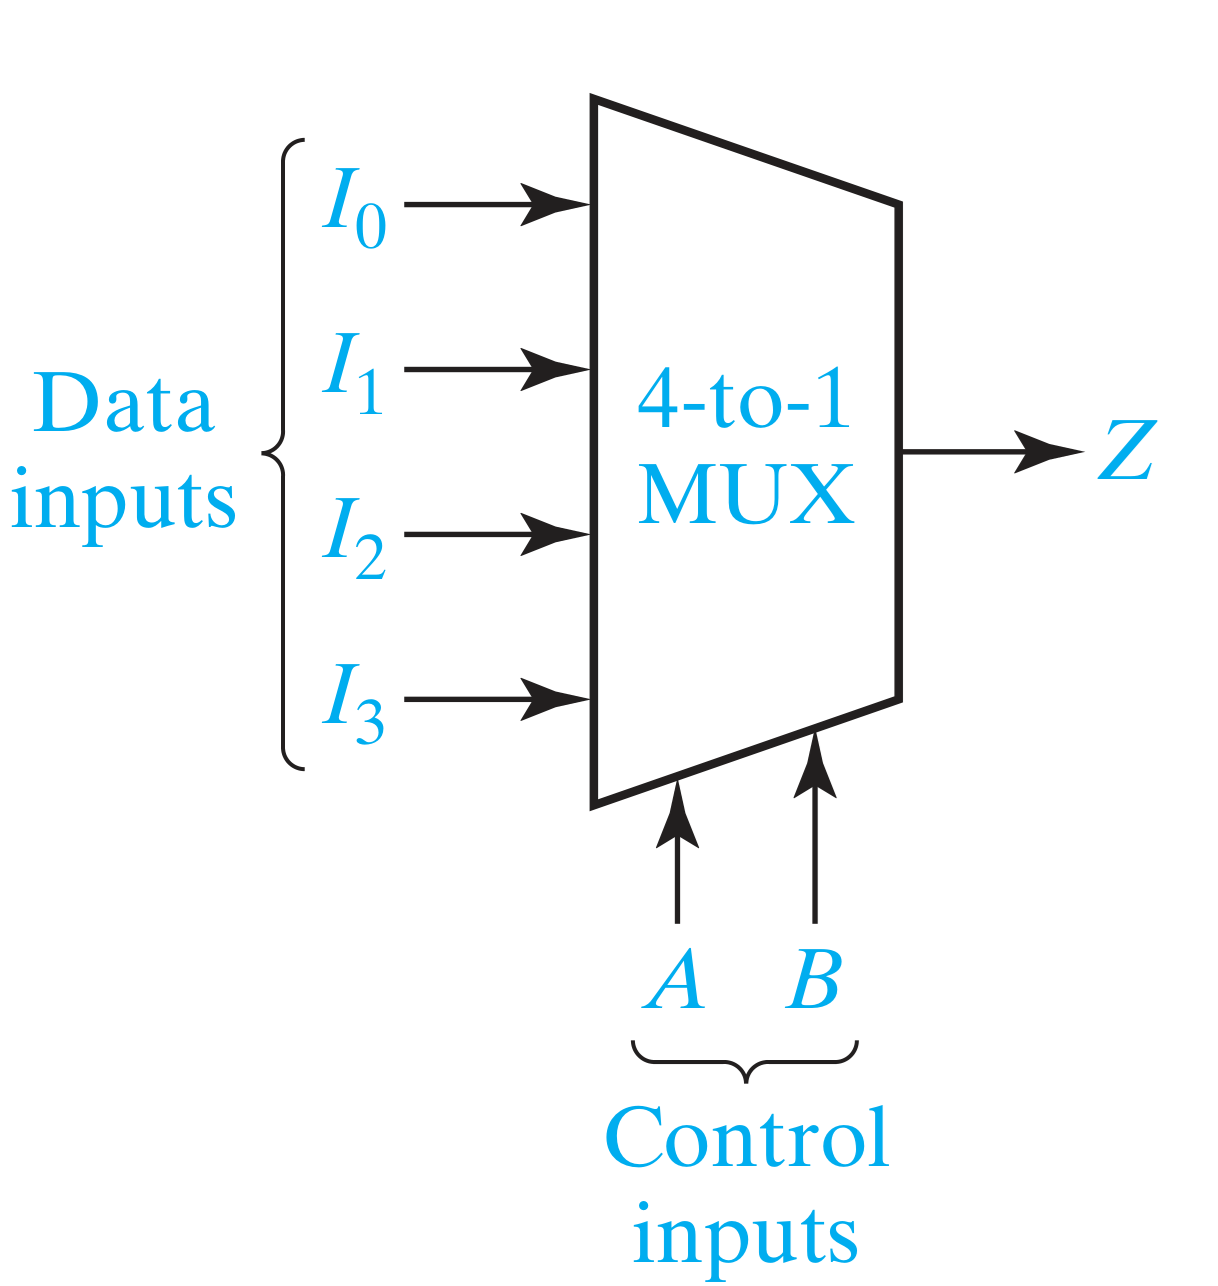
\includegraphics[scale=0.5]{examp081.png}}
	\captionof{figure}{4:1 MUX}
\end{figure}
Essentially, these IC's act as switches which select one of the inputs that is
connected to them. In general,

\textit{n} control inputs can be used to select one of \(2^n\) data inputs.
\[
	Z = \sum_{k=0}^{2^n-1} m_k \cdot I_k
\]
Where \(m_k\) is the k-th minterm of the select signals and \(I_k\) is the
respective data input.

The select lines can also be tied to a clock counter sort of signal in order to
cycle through the inputs. This is useful in analog circuits where a waveform can
be "compressed" into many cycles and decoded such that input 1 has a certain
frequency and amplitude and input 2 has another. This can introduce a lot of
noise however and makes it difficult to troubleshoot.

\subsubsection*{Why just half of a 74153?}
The lab has us design a circuit to implement two MUX's as a lookup table. In
this orientation, because each input MUX has two select states, and we only
utilize one output per MUX, we only need one of the two MUX's in the 74153.

Functionally, each pair of MUX's is abstracted into a 4 bit
selector.

Since we are using Shannon's expansion to convert the inputs to a function that
depends on the last input, each three person voting machine has select lines
assigned to two people, \(W\) and \(X\) in this case, and \(Y\) is used to be the
input to the mux as needed. By doing this, the inputs are limited to \(1, 0, Y
\) or  \(\overline{Y}\) and the output is a function of \(Y\).
\section*{Discussion}
\begin{examp}
	\vspace{.5cm}
	\textbf{A Three Person Voting Machine}
	\begin{enumerate}
		\item \textbf{Derive the Truth Table from the Inputs:}\\
		      Given the inputs, \(W (S_1) \quad X (S_0) \quad \text{and}\quad Y\),a standard
		      truth table is developed, with the output, \(F\) being the majority
		      vote outcome.
		      \(W\) and \(X\) were denoted \(S_1\) and \(S_0\) forward
		      thinking to the implementation.
		      \begin{table}[H]
			      \centering
			      \begin{tabular}{|c|c|c|c|}
				      \hline
				      \(W (S_1)\) & \(X (S_0)\) & \(Y\) & \(F\) \\
				      \hline
				      0           & 0           & 0     & 0     \\
				      0           & 0           & 1     & 0     \\
				      0           & 1           & 0     & 0     \\
				      0           & 1           & 1     & 1     \\
				      1           & 0           & 0     & 0     \\
				      1           & 0           & 1     & 1     \\
				      1           & 1           & 0     & 1     \\
				      1           & 1           & 1     & 1     \\
				      \hline
			      \end{tabular}
			      \caption{Voting Machine Logic}
		      \end{table}
		\item \textbf{Intuit the Design}\\
		      With the 4-1 MUX, we only have two select lines, so the classic
		      implementation where each select line ``selects" a specific output, the
		      complexity must be reduced from three to two.
		      Grouping the first two inputs \(S_1\) and \(S_0\) and making a fifth column which designates
		      our four inputs \(D_0\) \(D_1\) \(D_2\) and \(D_3\) allows this to be
		      done simply:
		      \begin{table}[H]
			      \centering
			      \begin{tabular}{|c|c|c|c|c|}
				      \hline
				      \(W (S_1)\)           & \(X (S_0)\) & \(Y\) & \(F\) & \(D_i\)                         \\
				      \hline
				      \rowcolor[gray]{.9}	0 & 0           & 0     & 0     & D\textsubscript{0} \textbf{= 0} \\
				      \rowcolor[gray]{.9}	0 & 0           & 1     & 0     & D\textsubscript{0} \textbf{= 0} \\
				      0                     & 1           & 0     & 0     & D\textsubscript{1} \textbf{= Y} \\
				      0                     & 1           & 1     & 1     & D\textsubscript{1} \textbf{= Y} \\
				      \rowcolor[gray]{.9}	1 & 0           & 0     & 0     & D\textsubscript{2} \textbf{= Y} \\
				      \rowcolor[gray]{.9}	1 & 0           & 1     & 1     & D\textsubscript{2} \textbf{= Y} \\
				      1                     & 1           & 0     & 1     & D\textsubscript{3} \textbf{= 1} \\
				      1                     & 1           & 1     & 1     & D\textsubscript{3} \textbf{= 1} \\
				      \hline
			      \end{tabular}
			      \caption{Simplified Voting Machine Logic}
		      \end{table}
		\item \textbf{Result}\\
		      This table shows that the inputs to the MUX can now be mapped to
		      either the third voter, \(Y\), Logic High, or Logic Low. This is exactly
		      what is needed for hardware implementation.
	\end{enumerate}
\end{examp}

\begin{examp}
	\subsubsection*{A 12-Person Voting Machine?}
	A almost identical approach was given to the expansion from three to 12 possible
	voters, but with an 8-1 MUX added at the final output.
	\begin{enumerate}
		\item \textbf{The 74151 MUX}\\
		      The 74151 MUX has \textit{three} select lines which can be mapped to
		      inputs. The problem is an expansion of the first in learning how to
		      get four seperate input logic inputs to a single output that represents a
		      majority vote.
		\item \textbf{The Select Lines}\\
		      In order to do this, the MUX from Part 1 is used as an input, signifying
		      the vote of a block of three voters.
		      If each block of three voters is an input, a logic table indicating the
		      results of these MUX's can be made and implemented
		\item \textbf{The Simplification}\\
		      The same simplification must occur. There are four inputs to be selected,
		      with only three select lines, so one of the inputs becomes the logic.
		      \begin{table}[H]
			      \centering
			      \begin{tabular}{|c|c|c|c|c|c|}
				      \hline
				      \(D (S_2)\)             & \(C (S_1)\) & \(B (S_0)\) & \(A\) & \(F\) & \(D_i\)                         \\
				      \hline
				      \rowcolor[gray]{.9} 0   & 0           & 0           & 0     & 0     & D\textsubscript{0} \textbf{= 0} \\
				      \rowcolor[gray]{.9}		0  & 0           & 0           & 1     & 0     & D\textsubscript{0} \textbf{= 0} \\
				      0                       & 0           & 1           & 0     & 0     & D\textsubscript{1} \textbf{= 0} \\
				      \rowcolor[gray]{.9} 0   & 0           & 1           & 1     & 0     & D\textsubscript{1} \textbf{= 0} \\
				      \rowcolor[gray]{.9} 		0 & 1           & 0           & 0     & 0     & D\textsubscript{2} \textbf{= 0} \\
				      0                       & 1           & 0           & 1     & 0     & D\textsubscript{2} \textbf{= 0} \\
				      \rowcolor[gray]{.9} 0   & 1           & 1           & 0     & 0     & D\textsubscript{3} \textbf{= A} \\
				      \rowcolor[gray]{.9} 0   & 1           & 1           & 1     & 1     & D\textsubscript{3} \textbf{= A} \\
				      \hline
				      1                       & 0           & 0           & 0     & 0     & D\textsubscript{4} \textbf{= 0} \\
				      1                       & 0           & 0           & 1     & 0     & D\textsubscript{4} \textbf{= 0} \\
				      \rowcolor[gray]{.9}  1  & 0           & 1           & 0     & 0     & D\textsubscript{5} \textbf{= A} \\
				      \rowcolor[gray]{.9}1    & 0           & 1           & 1     & 1     & D\textsubscript{5} \textbf{= A} \\
				      1                       & 1           & 0           & 0     & 0     & D\textsubscript{6} \textbf{= A} \\
				      1                       & 1           & 0           & 1     & 1     & D\textsubscript{6} \textbf{= A} \\
				      \rowcolor[gray]{.9}1    & 1           & 1           & 0     & 1     & D\textsubscript{7} \textbf{= 1} \\
				      \rowcolor[gray]{.9}		1  & 1           & 1           & 1     & 1     & D\textsubscript{7} \textbf{= 1} \\
				      \hline
			      \end{tabular}
			      \caption{12 Person Logic Table with MUX Inputs}
		      \end{table}
		\item \textbf{Result}\\
		      An reduction of what our data inputs to the 8:1 MUX is developed and easily
		      implementable in hardware with the three varying inputs \(0\) or Logic Low, \(A\), and \(1\) or
		      Logic High. The select lines input the logical outcome from the first
		      three voting machines.
	\end{enumerate}
\end{examp}

\section*{Practice Questions}
\begin{examp}
	\vspace{.5cm}
	\textbf{The Difference between Mealy and Moore Machines}\\
	In sequential logic, there are two ways to illustrate the forms of how a circuit
	operates called \textit{Finite State Machines}. These forms show the
	\textit{next state logic} and the \textit{output logic}.
	
	In general, a FSM contains \(2^k\) \textit{finite} output states such that
	there are \(M\) inputs, \(N\) outputs, and \(k\) bits of state.
	
	In a \textbf{Moore Machine}, the outputs depend exclusively on the \textit{current state} of the machine. This means that the output remains consistent as long as the system stays in a particular state, regardless of changes in the inputs. Consequently:
	\begin{itemize}
		\item \textbf{Predictable Outputs}: Because the outputs are tied solely to the state, they are stable and do not change unexpectedly due to momentary fluctuations in the inputs.
		\item \textbf{Design Simplicity}: A Moore Machine is often simpler to design because the output logic only needs to account for the state, not the inputs.
	\end{itemize}
	In contrast, a \textbf{Mealy Machine}’s outputs are determined by a combination of the \textit{current state} \textbf{and} the \textit{current input}. This makes the output sensitive to changes in the input, allowing for faster responses:
	
	\begin{itemize}
		\item \textbf{Responsive Outputs}: Since outputs are based on both the state and input, a Mealy Machine can react immediately to changes in inputs, making it more dynamic.
		      
		\item \textbf{Complexity}: The dual dependency on both inputs and state can make a Mealy Machine more complex to design and predict. However, it can also lead to fewer states being required, as the inputs directly influence the outputs.
	\end{itemize}
	
	The ticket-to-ride for this concept, is that Moore Machines only rely on
	Current State. Mealy Machines rely on Current State and the Input. This allows
	the Mealy Machine FSM to be one clock cycle ahead of the Moore since it
	actively senses the input.
	
\end{examp}

\begin{examp}
\vspace{.5cm}
\textbf{J-K Flip Flop Made from D Flip-Flop}\\
The \textit{J-K Flip-Flop} is an extended \textit{S-R Flip-Flop} which
attempts to solve the erroneous state in which both State and Reset are
Enabled.

This introduces a new ``Toggle" state in which on each clock pulse, the output
\(Q\) and \(\overline{Q}\) flip values.


\begin{figure}[H]
	\center{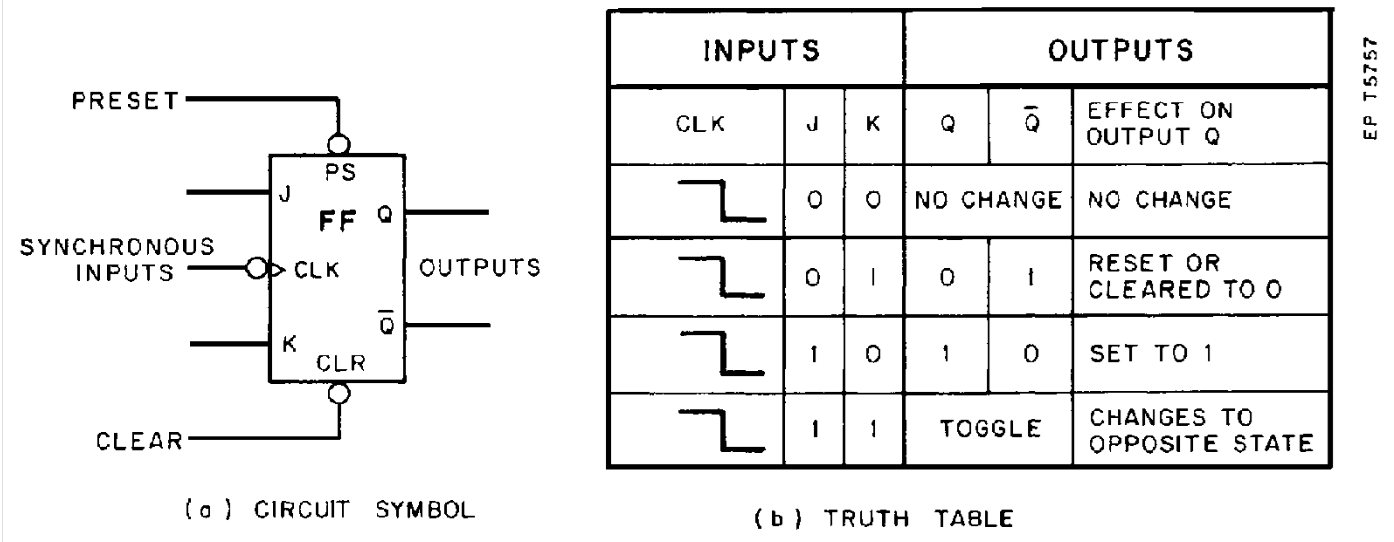
\includegraphics[scale=0.5]{examp084.png}}
	\captionof{figure}{The J-K Flip Flop}
\end{figure}

The \textit{D Flip-Flop} or \textit{Delay Flip-Flop} are widely used to form
shift or storage registers. This only has one data input \(D\), a clock CLK, and
the outputs \(Q\) and \(\overline{Q}\). But first, some terms to describe
these \textit{things}.
\begin{itemize}
	\item Transparent - When Data, \(D\) flows to Output \(Q\).
	\item Opaque - When Data, \(D\) is blocked from flowing and \(Q\) retains its
	      old value.
	\item Master (Leader) - When two back to back flip-flops or latches are
	      controlled by complimentary clocks and the output of the Master(Leader)
	      \(Q\) flows into the input of the Slave(Follower) \(D\)
	\item Slave (Follower) - The second latch or flip-flop in the complimentary clock
	      chain. This follows what the Master does.
	\item Edge-Triggered - When the rising or falling "edge" of a signal
	      causes the logic to advance
	\item Level-Triggered - When the input being high or low causes the signal
	      to advance. More in later example.
\end{itemize}
The D Flip Flop is just two D latches tied together which are simply SR
Latches that are clocked. More information on the distinction between these can
be found in the next example.

To convert from one to the other, the the table describing \(Q_n\), our
current state, and \(Q_{n+1}\), the next state is populated logically. This
will form the inputs to the D Flip-Flop. Recall that the J and K inputs
correspond to Set and Reset from the SR Latch.

\begin{table}[H]
	\centering
	\begin{tabular}{|c|c|c|c|c|}
		\hline
		\(Q_n\) & \(J\) & \(K\) & \(Q_{n+1}\) & \(D_i\) \\
		\hline
		0       & 0     & 0     & 0           & 0       \\
		0       & 0     & 1     & 0           & 0       \\
		0       & 1     & 0     & 1           & 1       \\
		0       & 1     & 1     & 1           & 1       \\
		1       & 0     & 0     & 1           & 1       \\
		1       & 0     & 1     & 0           & 0       \\
		1       & 1     & 0     & 1           & 1       \\
		1       & 1     & 1     & 0           & 0       \\
		\hline
	\end{tabular}
	\caption{Mapping J-K Logic to D Logic}
\end{table}

I use a Karnaugh Map to simplify this mapping:
\begin{center}
\begin{karnaugh-map}(label=corner)[4][2][1][$J$][$K$][$Q_n$]
\minterms{2,3,4,6}
\implicant{3}{2}
\implicantedge{4}{4}{6}{6}
\autoterms[0]
\end{karnaugh-map}
\end{center}
Therefore,
\[
	D = Q_n\overline{K} + \overline{Q_n}J
\]

\begin{figure}[H]
	\center{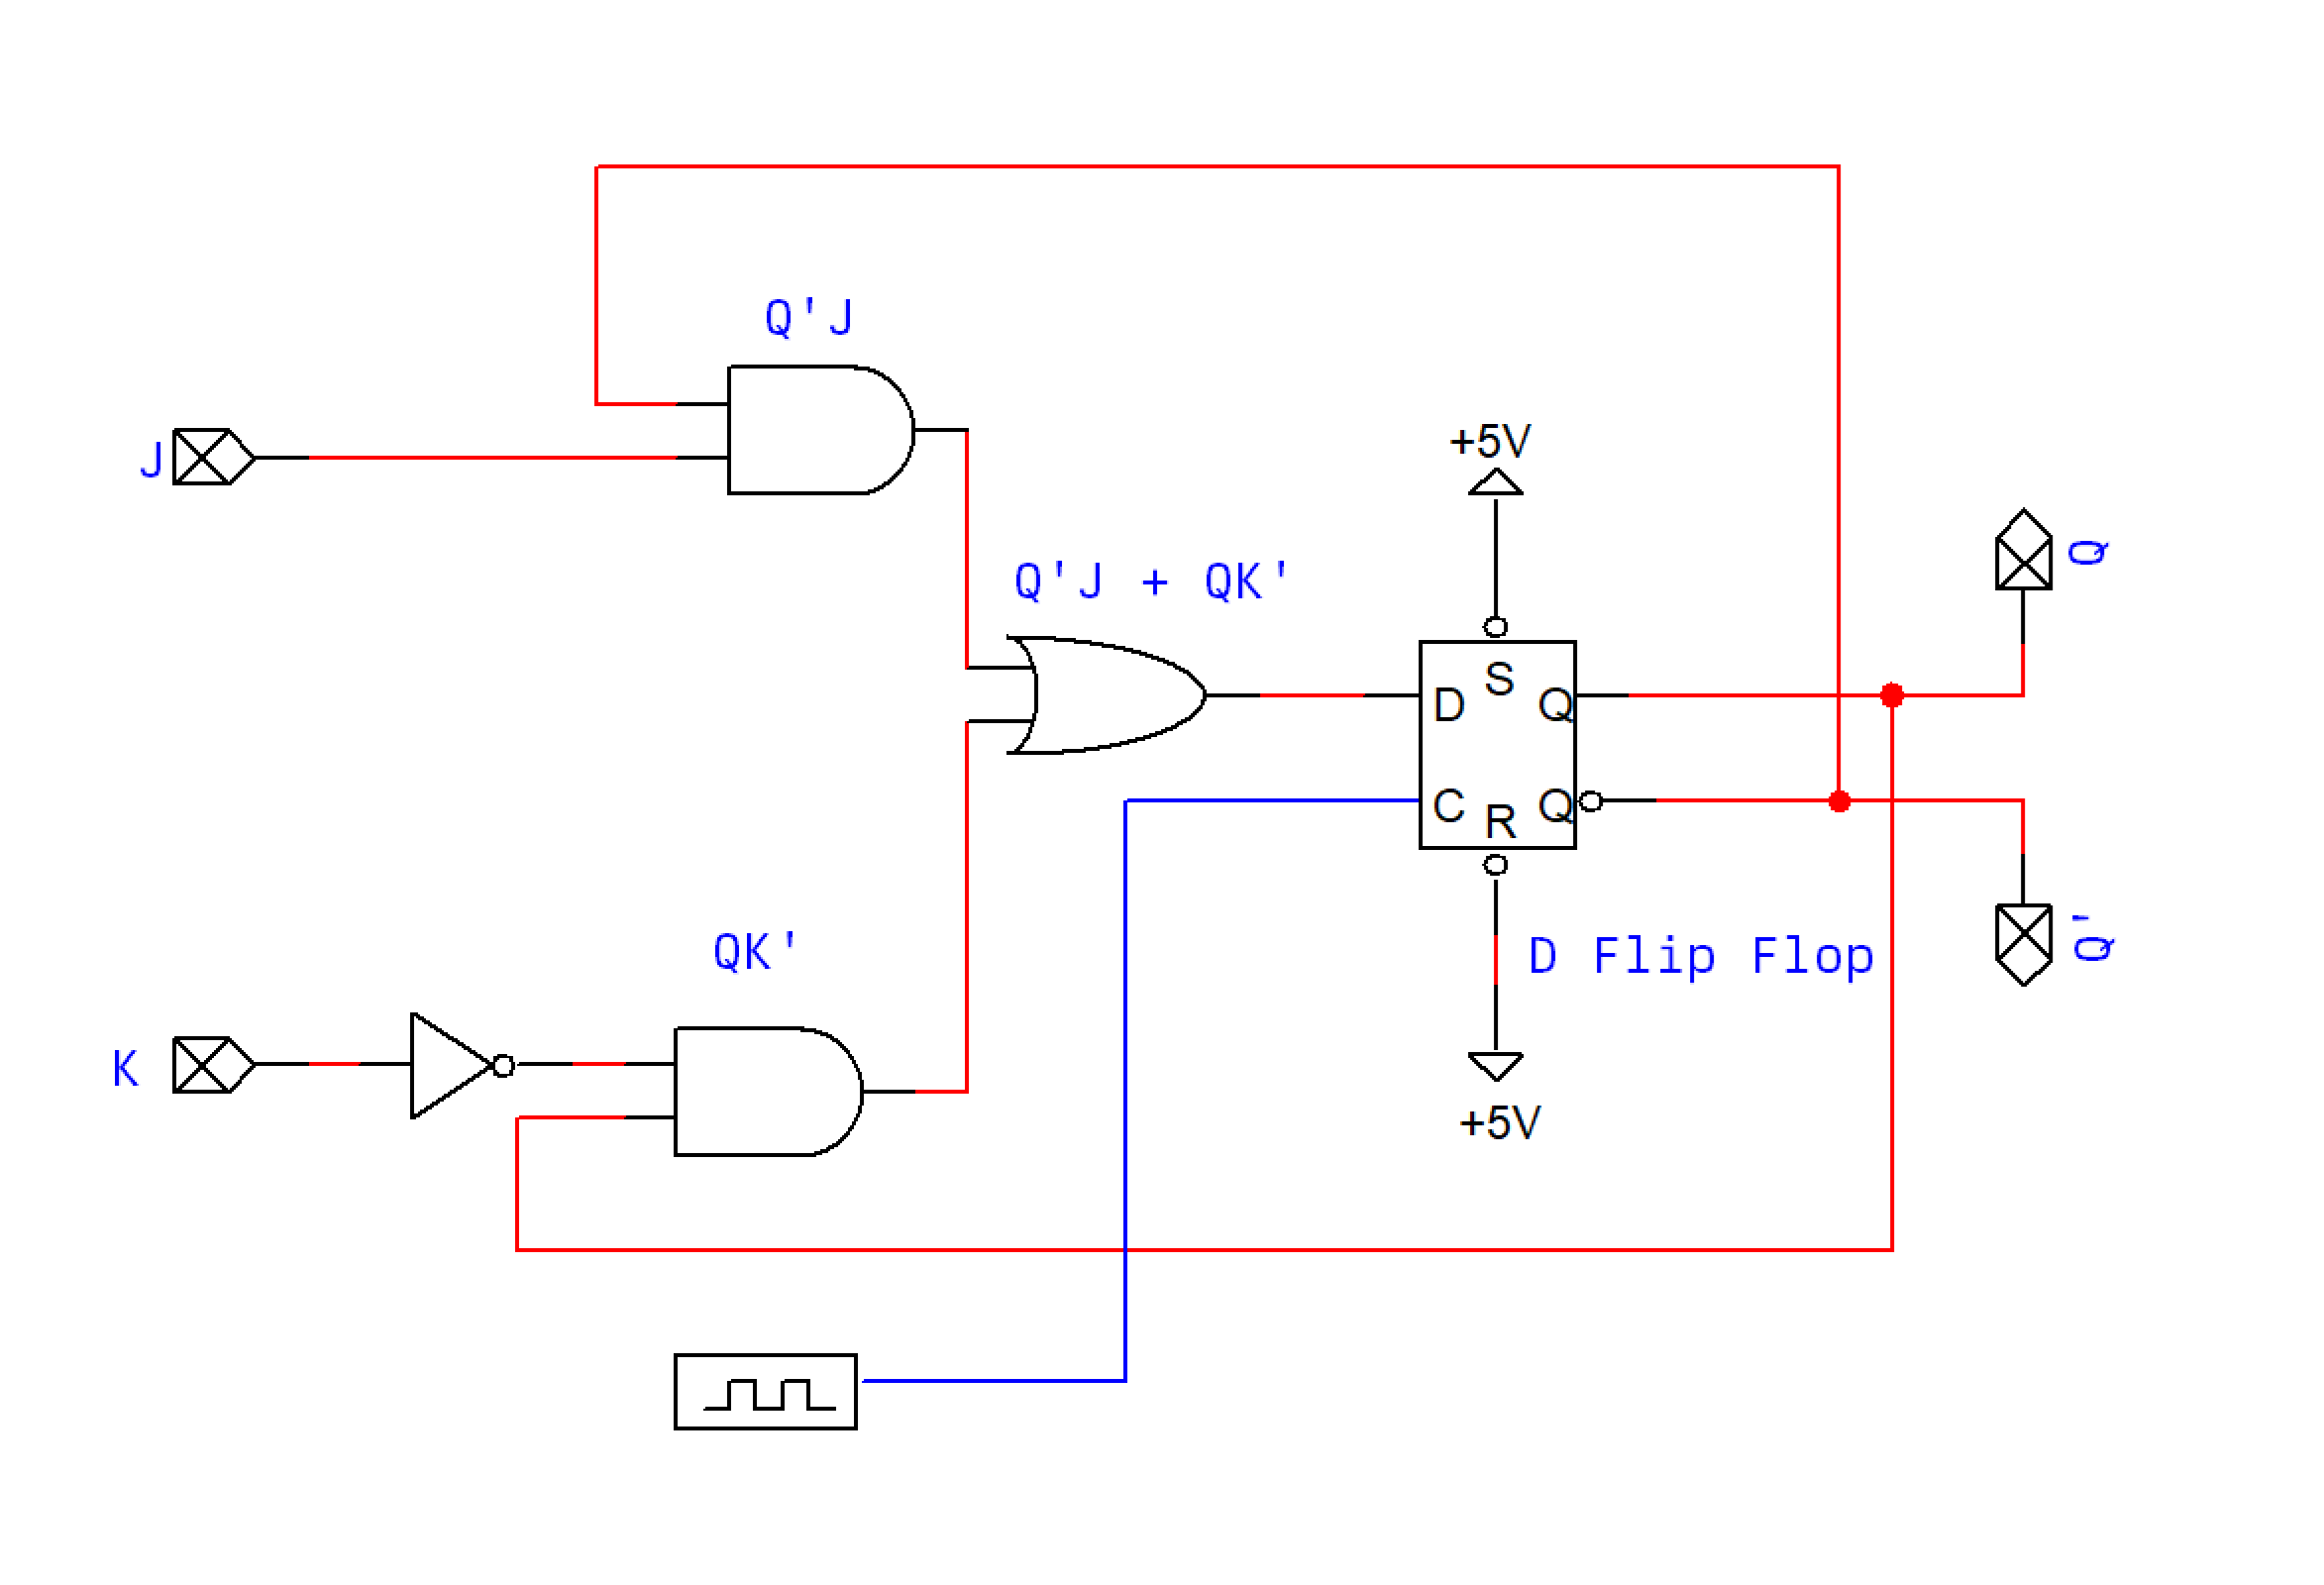
\includegraphics[scale=0.5]{examp083.png}}
	\captionof{figure}{The J-K Flip-Flop Implemented with D Flip-Flop}
\end{figure}
\end{examp}

\begin{examp}
	\textbf{Latch and Flip-Flops?}\\
	The main difference between any latch and any
	flip-flop is that the flip-flop is \textit{edge-triggered}.
	
	Edge-Triggered means that when a clock's rising or falling edge is felt on the circuitry, depending on whether it is positive or negative edge-triggered, triggers the data to flow and the Flip-Flop to be transparent.
	
	In general when
	not specified, it is assumed that a \textit{latch} and \textit{flip-flop}
	refers to a D flip-flop or a D latch.
	\begin{figure}[H]
		\centering
		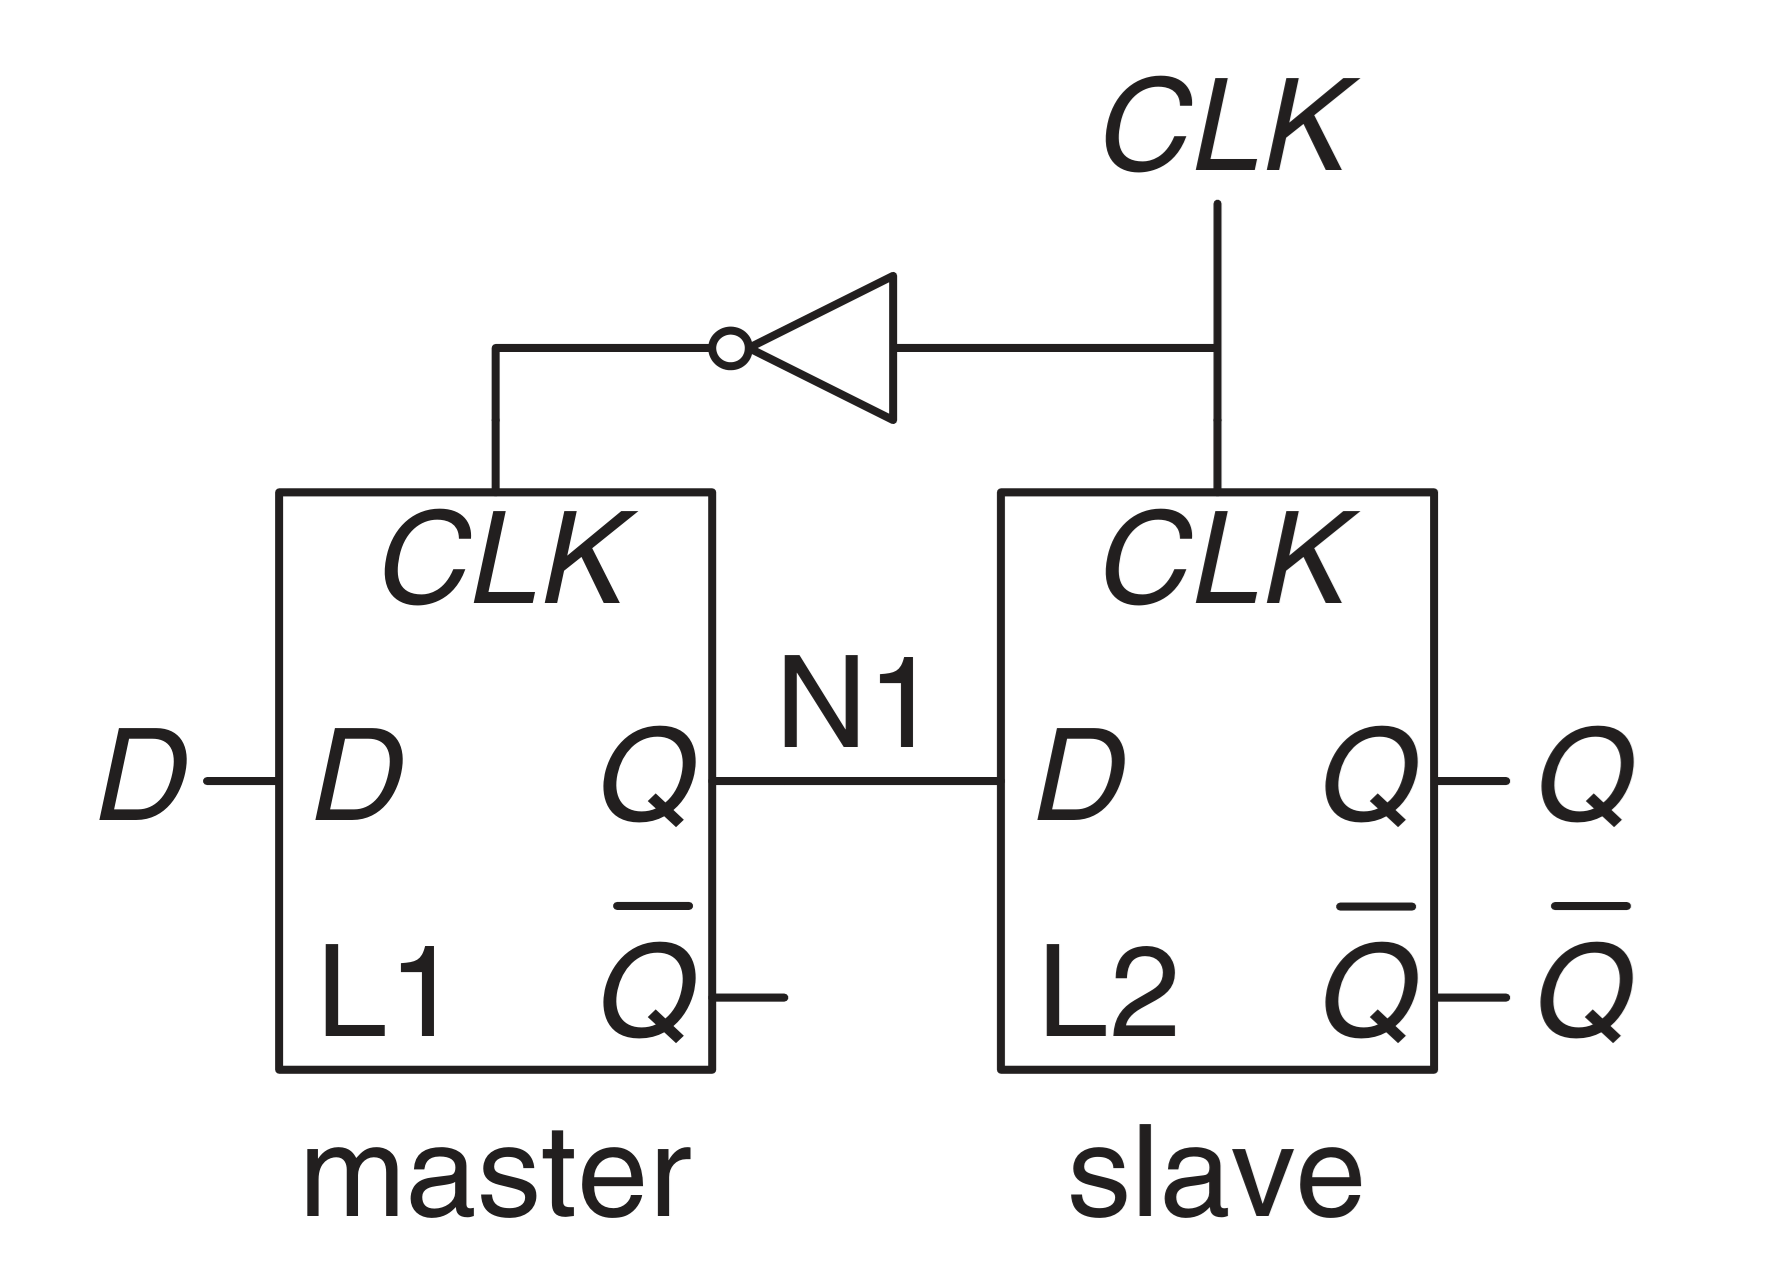
\includegraphics[scale=.3]{examp082.png}
		\captionof{figure}{A D Flip-Flop made from D Latches}
	\end{figure}
	\begin{enumerate}
		\item The Master is enabled during the clock's LOW phase.
		\item The Slave is enabled during the clock's HIGH phase.
	\end{enumerate}
	The primary difference between the two is:
	
	\begin{itemize}
		\item Latches are Level Triggered, not Edge-Triggered.
	\end{itemize}
	
	The complimentary clock pulse
	is tied to a slave and a master latch, which handle the pulse on different
	clock \textit{levels}. This can lead to buggy output behavior, so the
	Flip-Flop can precicely capture data at the clock edge.
	
	
\end{examp}

\end{document}
% vim: set tw=80 ts=2 sts=2 sw=2 noai noet:
